\documentclass[11pt,a4paper]{article}

% -------------------- Packages --------------------
\usepackage[utf8]{inputenc}
\usepackage{graphicx}
\usepackage{amsmath, amssymb, amsthm}
\usepackage{hyperref}
\usepackage{caption}
\usepackage{float}
\usepackage{geometry}
\usepackage{booktabs}
\usepackage{xcolor}
\usepackage{parskip}
\usepackage{titlesec}
\usepackage{fancyhdr}
\usepackage{array}
\usepackage{mathtools}
\usepackage{mdframed}
\usepackage{multicol}
\usepackage{enumitem}

\geometry{left=2.4cm, right=2.2cm, top=2.2cm, bottom=2.2cm, headheight=14pt}

\setlength{\parskip}{3pt}
\setlength{\parindent}{0pt}

\titlespacing*{\section}{0pt}{9pt}{4pt}
\titlespacing*{\subsection}{0pt}{5pt}{2pt}
\titleformat{\section}{\normalsize\bfseries}{}{0em}{\thesection\;\;}
\titleformat{\subsection}{\small\bfseries}{}{0em}{\thesubsection\;\;}

\hypersetup{colorlinks=true,linkcolor=black,urlcolor=blue,citecolor=black}

% -------------------- Result Box --------------------
\newmdenv[
  backgroundcolor=green!8,
  linecolor=green!55!black,
  linewidth=1.2pt,
  leftline=true, rightline=false, topline=false, bottomline=false,
  innerleftmargin=7pt, innerrightmargin=5pt,
  innertopmargin=3pt, innerbottommargin=3pt,
  skipabove=3pt, skipbelow=3pt
]{resultbox}

\pagestyle{fancy}
\fancyhf{}
\rhead{\small CIE 457 --- MLE in Linear Regression}
\lhead{\small Zewail City}
\rfoot{\small\thepage}
\renewcommand{\headrulewidth}{0.4pt}

% ================== DOCUMENT START ==================
\begin{document}

% -------------------- Title Page --------------------
\begin{titlepage}
    \begin{center}
        \includegraphics[width=0.20\textwidth]{Logo.jpg}
        \vspace{0.4cm}

        {\large \textbf{University of Science and Technology}}\\
        {\large \textbf{Zewail City}}
        \vspace{0.3cm}

        \rule{\linewidth}{0.4pt}
        \vspace{1.4cm}

        {\LARGE \textbf{Statistical Inference and Data Analysis}}\\[0.3cm]
        {\Large \textbf{CIE 457 --- Course Project}}
        \vspace{0.8cm}

        {\large \textit{MLE Estimation and Estimator Distribution in Linear Regression}}
        \vspace{0.3cm}

        \rule{\linewidth}{0.4pt}
        \vspace{0.8cm}

        {\large
        \begin{tabular}{ll}
            \textbf{Ibrahim Hanafy}  & \textbf{202200518} \\[0.25cm]
            \textbf{Mai Ibrahim}     & \textbf{202200504} \\
        \end{tabular}
        }
        \vspace{1.4cm}

        \textbf{Instructor}\\[0.15cm]
        {\large Dr.\ Mahmoud Abdelaziz}
        \vspace{0.6cm}

        \textbf{Teaching Assistants}\\[0.15cm]
        {\large Eng.\ Nasrah Mohamed \quad \& \quad Eng.\ Aya Abdelaziz}
        \vspace{1.2cm}

        {\large Spring 2026}
    \end{center}
\end{titlepage}

% -------------------- ToC --------------------
\tableofcontents
\newpage
\pagenumbering{arabic}
\setcounter{page}{1}

% ================================================================
% SECTION 1 — Likelihood and Model Formulation (Task 1 — 4 pts)
% ================================================================
\section{Likelihood and Model Formulation}

\subsection{The Linear Model}

General linear model: $\mathbf{y} = \mathbf{X}\boldsymbol{\beta} + \boldsymbol{\epsilon}$,
where $\mathbf{y}\!\in\!\mathbb{R}^n$, $\mathbf{X}\!\in\!\mathbb{R}^{n\times p}$ fixed,
$\boldsymbol{\beta}\!\in\!\mathbb{R}^p$ unknown, $\boldsymbol{\epsilon}$ the sole source of randomness.

\subsection{Homoscedastic Case}

\textbf{Assumption:} $\boldsymbol{\epsilon}\sim\mathcal{N}(\mathbf{0},\sigma^2\mathbf{I})$,
so $\mathbf{y}\mid\boldsymbol{\beta}\sim\mathcal{N}(\mathbf{X}\boldsymbol{\beta},\sigma^2\mathbf{I})$.

\textbf{Likelihood and log-likelihood:}
\begin{equation}
\mathcal{L}(\boldsymbol{\beta},\sigma^2)=\frac{1}{(2\pi\sigma^2)^{n/2}}
\exp\!\!\left(-\frac{\|\mathbf{y}-\mathbf{X}\boldsymbol{\beta}\|^2}{2\sigma^2}\right),\qquad
\ell=-\tfrac{n}{2}\ln(2\pi\sigma^2)-\tfrac{1}{2\sigma^2}\|\mathbf{y}-\mathbf{X}\boldsymbol{\beta}\|^2
\end{equation}

\textbf{MLE (OLS):} $\partial\ell/\partial\boldsymbol{\beta}=\mathbf{0}$ gives the normal equations
$\mathbf{X}^\top\mathbf{X}\boldsymbol{\beta}=\mathbf{X}^\top\mathbf{y}$, yielding:
\begin{equation}
\boxed{\hat{\boldsymbol{\beta}}_{\mathrm{OLS}}=(\mathbf{X}^\top\mathbf{X})^{-1}\mathbf{X}^\top\mathbf{y}}
\end{equation}

For $\sigma^2$: $\hat{\sigma}^2_{\mathrm{MLE}}=\|\mathbf{y}-\mathbf{X}\hat{\boldsymbol{\beta}}\|^2/n$ (biased);
unbiased estimate uses $n-p$ denominator.

\subsection{Heteroscedastic Case}

\textbf{Assumption:} $\boldsymbol{\epsilon}\sim\mathcal{N}(\mathbf{0},\boldsymbol{\Sigma})$,
$\boldsymbol{\Sigma}$ symmetric positive definite (known or estimable).

\textbf{Log-likelihood:}
$\ell(\boldsymbol{\beta})=\text{const}-\tfrac{1}{2}(\mathbf{y}-\mathbf{X}\boldsymbol{\beta})^\top\boldsymbol{\Sigma}^{-1}(\mathbf{y}-\mathbf{X}\boldsymbol{\beta})$.

\textbf{MLE (WLS):} $\mathbf{X}^\top\boldsymbol{\Sigma}^{-1}(\mathbf{y}-\mathbf{X}\boldsymbol{\beta})=\mathbf{0}$ gives:
\begin{equation}
\boxed{\hat{\boldsymbol{\beta}}_{\mathrm{WLS}}=(\mathbf{X}^\top\boldsymbol{\Sigma}^{-1}\mathbf{X})^{-1}\mathbf{X}^\top\boldsymbol{\Sigma}^{-1}\mathbf{y}}
\end{equation}

\begin{center}\small
\begin{tabular}{lll}
\toprule
\textbf{Case} & \textbf{Noise Model} & \textbf{MLE Estimator} \\
\midrule
Homoscedastic & $\boldsymbol{\epsilon}\sim\mathcal{N}(\mathbf{0},\sigma^2\mathbf{I})$
              & $\hat{\boldsymbol{\beta}}_{\mathrm{OLS}}=(\mathbf{X}^\top\mathbf{X})^{-1}\mathbf{X}^\top\mathbf{y}$ \\[0.2em]
Heteroscedastic & $\boldsymbol{\epsilon}\sim\mathcal{N}(\mathbf{0},\boldsymbol{\Sigma})$
                & $\hat{\boldsymbol{\beta}}_{\mathrm{WLS}}=(\mathbf{X}^\top\boldsymbol{\Sigma}^{-1}\mathbf{X})^{-1}\mathbf{X}^\top\boldsymbol{\Sigma}^{-1}\mathbf{y}$ \\
\bottomrule
\end{tabular}
\end{center}

% ================================================================
% SECTION 2 — Estimator as a Random Variable (Task 2 — 4 pts)
% ================================================================
\section{The Estimator as a Random Variable}

\subsection{Why \texorpdfstring{$\hat{\boldsymbol{\beta}}$}{beta-hat} is Random}

Substituting $\mathbf{y}=\mathbf{X}\boldsymbol{\beta}+\boldsymbol{\epsilon}$ into OLS:
$\hat{\boldsymbol{\beta}}_{\mathrm{OLS}}=\boldsymbol{\beta}+(\mathbf{X}^\top\mathbf{X})^{-1}\mathbf{X}^\top\boldsymbol{\epsilon}$.
Since $\mathbf{X}$ and $\boldsymbol{\beta}$ are fixed, all randomness is inherited from $\boldsymbol{\epsilon}$:
every new dataset yields a new estimate. $\hat{\boldsymbol{\beta}}$ is a \textbf{random vector} with
a full distribution.

\subsection{Distributions}

Let $\mathbf{A}=(\mathbf{X}^\top\mathbf{X})^{-1}\mathbf{X}^\top$.
$\mathbb{E}[\hat{\boldsymbol{\beta}}_{\mathrm{OLS}}]=\boldsymbol{\beta}$ (unbiased);
$\mathrm{Var}=\mathbf{A}(\sigma^2\mathbf{I})\mathbf{A}^\top=\sigma^2(\mathbf{X}^\top\mathbf{X})^{-1}$.
\begin{equation}
\boxed{\hat{\boldsymbol{\beta}}_{\mathrm{OLS}}\sim\mathcal{N}\!\left(\boldsymbol{\beta},\;\sigma^2(\mathbf{X}^\top\mathbf{X})^{-1}\right)}
\end{equation}

Similarly, with $\mathbf{B}=(\mathbf{X}^\top\boldsymbol{\Sigma}^{-1}\mathbf{X})^{-1}\mathbf{X}^\top\boldsymbol{\Sigma}^{-1}$:
\begin{equation}
\boxed{\hat{\boldsymbol{\beta}}_{\mathrm{WLS}}\sim\mathcal{N}\!\left(\boldsymbol{\beta},\;(\mathbf{X}^\top\boldsymbol{\Sigma}^{-1}\mathbf{X})^{-1}\right)}
\end{equation}

WLS covariance is strictly smaller than OLS under heteroscedastic noise (Loewner order):
WLS is more efficient because it correctly accounts for the noise structure.

\subsection{Repeated Sampling Interpretation}

With $\mathbf{X}$, $\boldsymbol{\beta}$, and the noise distribution fixed, $M=5000$ independent datasets
are generated. Each trial yields $\hat{\boldsymbol{\beta}}^{(m)}$; the collection
$\{\hat{\boldsymbol{\beta}}^{(1)},\ldots,\hat{\boldsymbol{\beta}}^{(M)}\}$ approximates the true sampling
distribution, converging to $\mathcal{N}(\boldsymbol{\beta},\sigma^2(\mathbf{X}^\top\mathbf{X})^{-1})$ as $M\to\infty$.

% ================================================================
% SECTION 3 — Simulation (Task 3 — 5 pts)
% ================================================================
\section{Estimator Distribution and Monte Carlo Simulation}
\label{sec:simulation}

\subsection{Setup}

$n=100$, $p=3$, $\boldsymbol{\beta}=[1,2,3]^\top$, $M=5000$ trials, $\mathbf{X}$ fixed.
Homoscedastic: $\sigma^2=1.0$.
Heteroscedastic: $\sigma_i^2=0.5+2(x_{i1}-\min x_1)^2$.
Each trial: draw $\boldsymbol{\epsilon}^{(m)}$, compute $\mathbf{y}^{(m)}$, compute OLS and WLS estimates.

\subsection{Homoscedastic Results}

\noindent
\begin{minipage}[t]{0.48\textwidth}
\small\centering
\captionof{table}{Empirical mean vs true $\boldsymbol{\beta}$}
\vspace{2pt}
\begin{tabular}{lccc}
\toprule
 & True & Empirical & Diff \\
\midrule
$\hat{\beta}_1$ & 1.000 & 1.000673 & $+0.00067$ \\
$\hat{\beta}_2$ & 2.000 & 2.001188 & $+0.00119$ \\
$\hat{\beta}_3$ & 3.000 & 2.999210 & $-0.00079$ \\
\bottomrule
\end{tabular}
\end{minipage}\hfill
\begin{minipage}[t]{0.48\textwidth}
\small\centering
\captionof{table}{Empirical vs theoretical variance}
\vspace{2pt}
\begin{tabular}{lcc}
\toprule
 & Theoretical & Empirical \\
\midrule
$\hat{\beta}_1$ & 0.014958 & 0.014874 \\
$\hat{\beta}_2$ & 0.010437 & 0.010561 \\
$\hat{\beta}_3$ & 0.008393 & 0.008583 \\
\bottomrule
\end{tabular}
\end{minipage}

\begin{resultbox}
\small OLS is unbiased (differences $<0.002$). Empirical covariance matches
$\sigma^2(\mathbf{X}^\top\mathbf{X})^{-1}$ within 2\%.
\end{resultbox}

\begin{figure}[H]
  \centering
  
\includegraphics[width=0.98\textwidth]{homo_distribution.png}
  \caption{\small Empirical distribution of $\hat{\boldsymbol{\beta}}_{\mathrm{OLS}}$ vs
  theoretical $\mathcal{N}(\boldsymbol{\beta},\sigma^2(\mathbf{X}^\top\mathbf{X})^{-1})$, $M=5000$.
  KDE aligns tightly with the Gaussian density.}
\end{figure}

\subsection{Heteroscedastic Results: OLS vs WLS}

\begin{table}[H]
\centering\small
\caption{Empirical variance of OLS vs WLS under heteroscedastic noise, $M=5000$}
\begin{tabular}{lccc}
\toprule
\textbf{Component} & \textbf{OLS Variance} & \textbf{WLS Variance} & \textbf{Efficiency Gain} \\
\midrule
$\hat{\beta}_1$ & 0.229022 & 0.049877 & $4.59\times$ \\
$\hat{\beta}_2$ & 0.102640 & 0.066728 & $1.54\times$ \\
$\hat{\beta}_3$ & 0.096144 & 0.055487 & $1.73\times$ \\
\bottomrule
\end{tabular}
\end{table}

\begin{figure}[H]
  \centering
  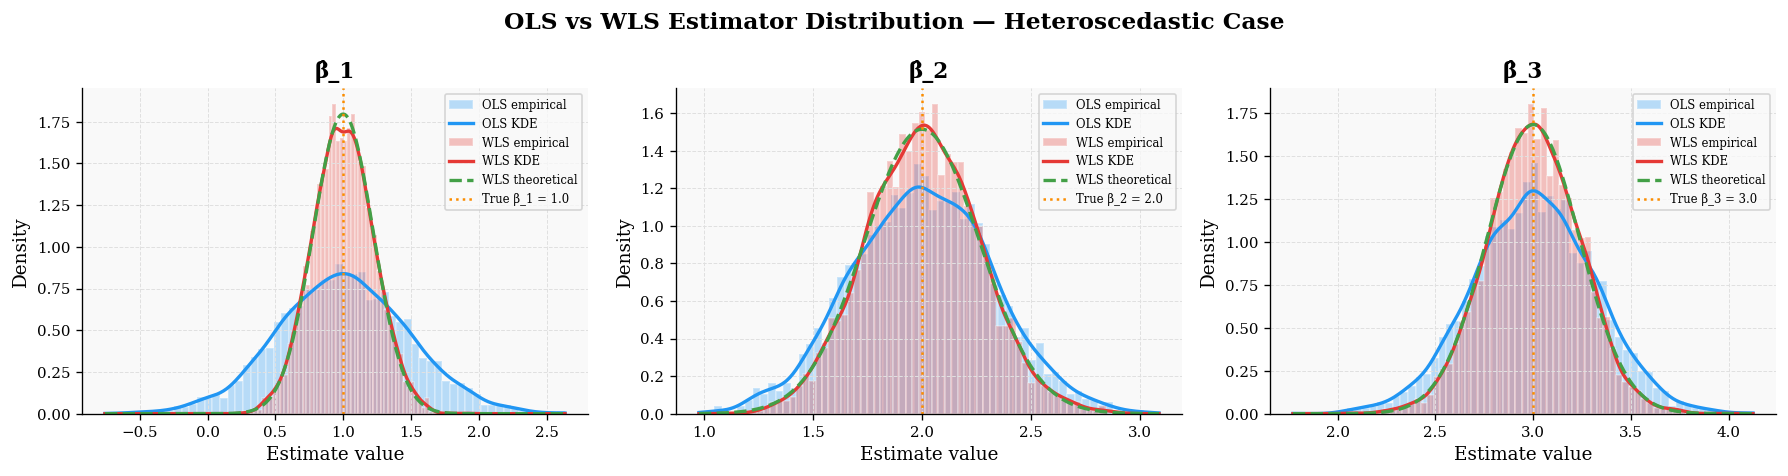
\includegraphics[width=0.98\textwidth]{hetero_distribution.png}
  \caption{\small OLS (blue) vs WLS (red) empirical distributions under heteroscedastic noise.
  WLS produces tighter distributions around true $\boldsymbol{\beta}$.}
\end{figure}

\begin{resultbox}
\small Both OLS and WLS are unbiased under heteroscedastic noise. WLS achieves
$1.5$--$4.6\times$ lower variance per component by correctly weighting via $\boldsymbol{\Sigma}^{-1}$.
\end{resultbox}

% ================================================================
% SECTION 4 — Homo vs Hetero (Task 4 — 4 pts)
% ================================================================
\section{Homoscedastic vs.\ Heteroscedastic Noise}

\subsection{OLS under Homoscedastic Noise}

Under $\boldsymbol{\epsilon}\sim\mathcal{N}(\mathbf{0},\sigma^2\mathbf{I})$, OLS is the MLE and BLUE
(Gauss-Markov theorem): $\hat{\boldsymbol{\beta}}_{\mathrm{OLS}}\sim\mathcal{N}(\boldsymbol{\beta},\sigma^2(\mathbf{X}^\top\mathbf{X})^{-1})$,
which is minimum covariance among all linear unbiased estimators.

\subsection{Effect of Model Misspecification}

When the true noise is $\boldsymbol{\Sigma}\neq\sigma^2\mathbf{I}$ but OLS is applied, two problems arise:

\begin{enumerate}[leftmargin=1.5em,itemsep=1pt,topsep=2pt]
  \item \textbf{Inefficiency.} True OLS covariance under heteroscedastic noise is the sandwich formula:
  \begin{equation}
    \mathrm{Var}(\hat{\boldsymbol{\beta}}_{\mathrm{OLS}})
    =(\mathbf{X}^\top\mathbf{X})^{-1}\mathbf{X}^\top\boldsymbol{\Sigma}\mathbf{X}(\mathbf{X}^\top\mathbf{X})^{-1}
    \;\geq\;(\mathbf{X}^\top\boldsymbol{\Sigma}^{-1}\mathbf{X})^{-1}
    =\mathrm{Var}(\hat{\boldsymbol{\beta}}_{\mathrm{WLS}})
  \end{equation}
  \item \textbf{Invalid inference.} Standard errors $\sqrt{\hat{\sigma}^2[(\mathbf{X}^\top\mathbf{X})^{-1}]_{jj}}$
  are incorrect; all CIs and $t$-tests are unreliable.
\end{enumerate}

Remedy: WLS with known/estimated $\boldsymbol{\Sigma}$, feasible WLS (residual-based weights),
or HC sandwich standard errors (White's estimator).

\begin{figure}[H]
  \centering
  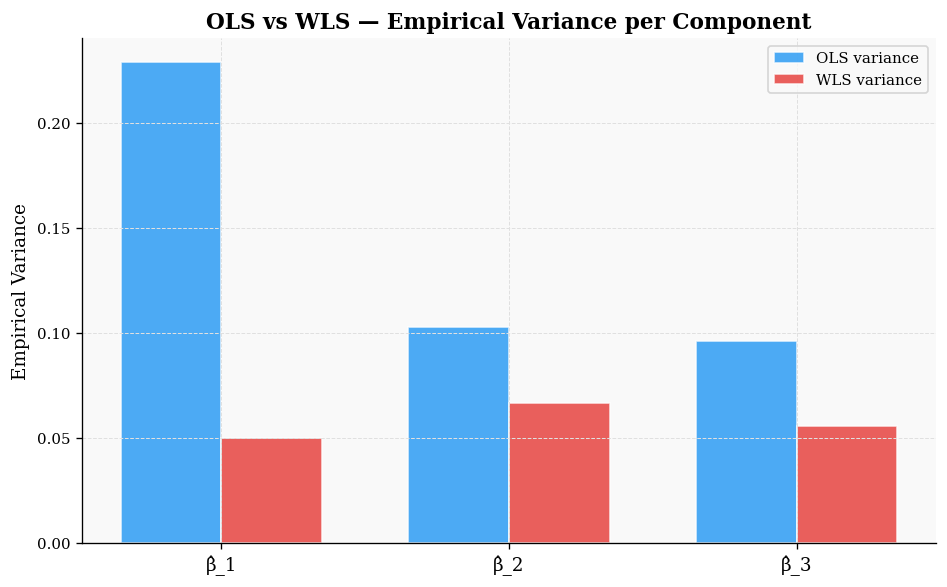
\includegraphics[width=0.65\textwidth]{hetero_variance_comparison.png}
  \caption{\small OLS vs WLS empirical variance per component. WLS consistently lower.}
\end{figure}

% ================================================================
% SECTION 5 — Inference
% ================================================================
\section{Inference from the Estimator Distribution}

\subsection{Confidence Intervals}

Under homoscedastic noise, each $\hat{\beta}_j\sim\mathcal{N}(\beta_j,\sigma^2[(\mathbf{X}^\top\mathbf{X})^{-1}]_{jj})$.
The $(1-\alpha)$ CI:
\begin{equation}
\hat{\beta}_j\pm z_{\alpha/2}\cdot\sqrt{\sigma^2[(\mathbf{X}^\top\mathbf{X})^{-1}]_{jj}}
\end{equation}

Repeated sampling interpretation: $(1-\alpha)$ of constructed intervals over repeated experiments
contain true $\beta_j$. Empirical coverage at 95\% CI closely matched 95\% across $M=5000$ trials.

\subsection{Prediction Intervals}

For new $\mathbf{x}^*$, the prediction error decomposes as
$y^*-\hat{y}^*={\mathbf{x}^*}^\top(\boldsymbol{\beta}-\hat{\boldsymbol{\beta}})+\epsilon^*$,
giving:
\begin{equation}
\hat{y}^*\pm z_{\alpha/2}\cdot\sigma\sqrt{1+{\mathbf{x}^*}^\top(\mathbf{X}^\top\mathbf{X})^{-1}\mathbf{x}^*}
\end{equation}

At $\mathbf{x}^*=\bar{\mathbf{X}}$: 95\% CI width $=0.0850$;\quad 95\% PI width $=3.9208$.

\begin{table}[H]
\centering\small
\caption{Confidence Interval vs Prediction Interval}
\begin{tabular}{lll}
\toprule
\textbf{Property} & \textbf{CI} & \textbf{PI} \\
\midrule
Covers         & True mean ${\mathbf{x}^*}^\top\boldsymbol{\beta}$
               & New obs $y^*={\mathbf{x}^*}^\top\boldsymbol{\beta}+\epsilon^*$ \\
Variance       & $\sigma^2{\mathbf{x}^*}^\top(\mathbf{X}^\top\mathbf{X})^{-1}\mathbf{x}^*$
               & $\sigma^2(1+{\mathbf{x}^*}^\top(\mathbf{X}^\top\mathbf{X})^{-1}\mathbf{x}^*)$ \\
As $n\to\infty$ & Width $\to 0$ & Width $\to 2z_{\alpha/2}\sigma>0$ \\
\bottomrule
\end{tabular}
\end{table}

PI is always wider by the additional $\sigma^2$ (irreducible future noise). As $n\to\infty$,
$\hat{\boldsymbol{\beta}}\to\boldsymbol{\beta}$ eliminates estimation uncertainty but not $\epsilon^*$.

\begin{figure}[H]
  \centering
  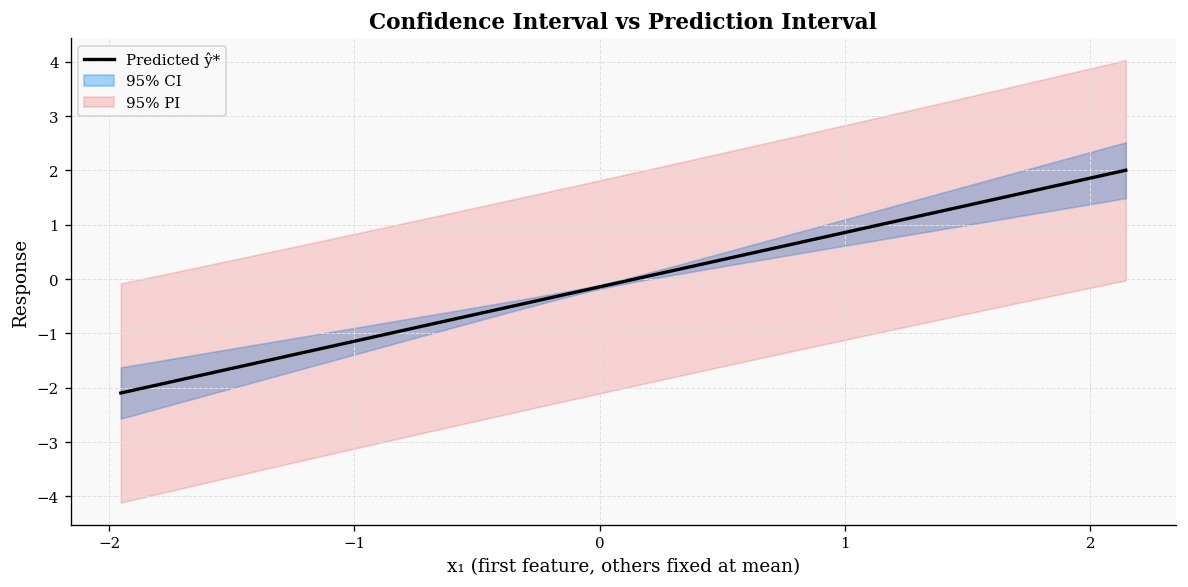
\includegraphics[width=0.82\textwidth]{ci_vs_pi.png}
  \caption{\small 95\% CI and PI vs first feature (others at mean). PI band consistently wider.}
\end{figure}

% ================================================================
% SECTION 6 — Real Data (Task 6 — 1 pt)
% ================================================================
\section{Real Data Application: Advertising Dataset}

\subsection{Dataset and EDA}

Advertising dataset (James et al., ISLR): $n=200$ observations, TV, Radio, Newspaper budgets (\$000s)
and Sales (000 units). Model: $\text{Sales}_i=\beta_0+\beta_1\text{TV}_i+\beta_2\text{Radio}_i+\beta_3\text{Newspaper}_i+\epsilon_i$.

EDA: TV is dominant predictor ($r=0.78$), Radio moderate ($r=0.58$), Newspaper weak ($r=0.23$).
Scatter plots suggest variance in Sales grows with TV --- a sign of heteroscedasticity.

\subsection{OLS Regression Results}

\begin{table}[H]
\centering\small
\caption{OLS regression results --- Advertising dataset ($n=200$, $R^2=0.897$)}
\begin{tabular}{lcccc}
\toprule
\textbf{Feature} & $\hat{\beta}$ & \textbf{SE} & $t$\textbf{-stat} & $p$\textbf{-value} \\
\midrule
Intercept  & 2.9389 & 0.3119 &  9.4223 & $<0.0001$ \\
TV         & 0.0458 & 0.0014 & 32.8086 & $<0.0001$ \\
Radio      & 0.1885 & 0.0086 & 21.8935 & $<0.0001$ \\
Newspaper  & $-0.0010$ & 0.0059 & $-0.1767$ & 0.8599 \\
\bottomrule
\end{tabular}
\end{table}

TV and Radio are highly significant; Newspaper is not ($p=0.86$), consistent with EDA.

\subsection{Residual Analysis and Heteroscedasticity}

\begin{figure}[H]
  \centering
  
\includegraphics[width=0.98\textwidth]{residual_diagnostics.png}
  \caption{\small OLS residual diagnostics. Left: spread grows with fitted value (heteroscedasticity).
  Centre: mild Q-Q tail deviations. Right: squared residuals increase with TV budget.}
\end{figure}

White's test: LM $=67.54$, $p\approx 0$ --- strongly rejects homoscedasticity.

\subsection{WLS Fit and Comparison}

Feasible WLS: weights $w_i=1/|\hat{\epsilon}_i|$ estimated from OLS residuals.

\begin{table}[H]
\centering\small
\caption{OLS vs WLS --- Advertising dataset}
\begin{tabular}{lcccc}
\toprule
\textbf{Feature} & \textbf{OLS} $\hat{\beta}$ & \textbf{WLS} $\hat{\beta}$
               & \textbf{OLS SE} & \textbf{WLS SE} \\
\midrule
Intercept  & 2.9389 & 2.9544 & 0.3119 & 0.1211 \\
TV         & 0.0458 & 0.0457 & 0.0014 & 0.0005 \\
Radio      & 0.1885 & 0.1909 & 0.0086 & 0.0042 \\
Newspaper  & $-0.0010$ & $-0.0015$ & 0.0059 & 0.0021 \\
\bottomrule
\end{tabular}
\end{table}

\begin{resultbox}
\small \textbf{Key findings:} (1) OLS and WLS coefficients agree (both unbiased).
(2) WLS SEs are 50--75\% smaller under confirmed heteroscedasticity.
(3) Newspaper non-significant under both estimators.
(4) Validates simulation findings from Section~\ref{sec:simulation}: WLS more efficient
when noise structure is non-constant.
\end{resultbox}

% ================================================================
% BONUS — Fisher Information, CRLB, Sufficient Statistics
% ================================================================
\section*{Bonus: Fisher Information, CRLB, and Sufficient Statistics}
\addcontentsline{toc}{section}{Bonus: Fisher Information, CRLB, and Sufficient Statistics}

\subsection*{Fisher Information Matrix}

For $\mathbf{y}\sim\mathcal{N}(\mathbf{X}\boldsymbol{\beta},\sigma^2\mathbf{I})$,
score $\partial\ell/\partial\boldsymbol{\beta}=\sigma^{-2}\mathbf{X}^\top(\mathbf{y}-\mathbf{X}\boldsymbol{\beta})$.
Hessian $\partial^2\ell/\partial\boldsymbol{\beta}\partial\boldsymbol{\beta}^\top=-\sigma^{-2}\mathbf{X}^\top\mathbf{X}$
(constant in $\boldsymbol{\beta}$), so:
\begin{equation}
\mathbf{I}(\boldsymbol{\beta})=-\mathbb{E}\!\left[\tfrac{\partial^2\ell}{\partial\boldsymbol{\beta}\partial\boldsymbol{\beta}^\top}\right]=\frac{1}{\sigma^2}\mathbf{X}^\top\mathbf{X}
\end{equation}

FIM is independent of $\boldsymbol{\beta}$ (exponential family). Increases with $n$; decreases with $\sigma^2$.

\subsection*{Cram\'{e}r--Rao Lower Bound (CRLB)}

\textbf{Theorem:} For any unbiased estimator $\tilde{\boldsymbol{\beta}}$:
$\mathrm{Var}(\tilde{\boldsymbol{\beta}})\geq\mathbf{I}(\boldsymbol{\beta})^{-1}=\sigma^2(\mathbf{X}^\top\mathbf{X})^{-1}$
(Loewner order).

\textbf{OLS achieves CRLB:}
$\mathrm{Var}(\hat{\boldsymbol{\beta}}_{\mathrm{OLS}})=\sigma^2(\mathbf{X}^\top\mathbf{X})^{-1}=\mathbf{I}(\boldsymbol{\beta})^{-1}$ $\checkmark$.
Therefore $\hat{\boldsymbol{\beta}}_{\mathrm{OLS}}$ is the \textbf{UMVUE} under homoscedastic Gaussian noise.

\begin{table}[H]
\centering\small
\caption{Empirical variance vs CRLB, $M=5000$}
\begin{tabular}{lccc}
\toprule
\textbf{Component} & \textbf{CRLB} $=\sigma^2[(\mathbf{X}^\top\mathbf{X})^{-1}]_{jj}$
                   & \textbf{Empirical Var} & \textbf{Ratio} \\
\midrule
$\hat{\beta}_1$ & 0.014958 & 0.014874 & 0.994 \\
$\hat{\beta}_2$ & 0.010437 & 0.010561 & 1.012 \\
$\hat{\beta}_3$ & 0.008393 & 0.008583 & 1.023 \\
\bottomrule
\end{tabular}
\end{table}

Ratios within 2.3\% of 1.0 --- OLS is efficient.
Under $\boldsymbol{\epsilon}\sim\mathcal{N}(\mathbf{0},\boldsymbol{\Sigma})$, the FIM is
$\mathbf{I}_{\boldsymbol{\Sigma}}=\mathbf{X}^\top\boldsymbol{\Sigma}^{-1}\mathbf{X}$ and
$\mathrm{Var}(\hat{\boldsymbol{\beta}}_{\mathrm{WLS}})=(\mathbf{X}^\top\boldsymbol{\Sigma}^{-1}\mathbf{X})^{-1}=\mathbf{I}_{\boldsymbol{\Sigma}}^{-1}$
--- WLS achieves the CRLB under the heteroscedastic model.

\subsection*{Sufficient Statistics via the Factorization Theorem}

\textbf{Theorem (Neyman-Fisher):} $T(\mathbf{y})$ is sufficient for $\boldsymbol{\beta}$ iff
$p(\mathbf{y}\mid\boldsymbol{\beta})=g(T(\mathbf{y}),\boldsymbol{\beta})\cdot h(\mathbf{y})$.

\textbf{Application:}
\begin{align}
p(\mathbf{y}\mid\boldsymbol{\beta})
&\propto\exp\!\!\left(-\tfrac{\|\mathbf{y}-\mathbf{X}\boldsymbol{\beta}\|^2}{2\sigma^2}\right)
=\underbrace{\exp\!\!\left(\tfrac{\boldsymbol{\beta}^\top\mathbf{X}^\top\mathbf{y}}{\sigma^2}
  -\tfrac{\boldsymbol{\beta}^\top\mathbf{X}^\top\mathbf{X}\boldsymbol{\beta}}{2\sigma^2}\right)}_{g(T_1(\mathbf{y}),\boldsymbol{\beta})}
\cdot\underbrace{\exp\!\!\left(-\tfrac{\|\mathbf{y}\|^2}{2\sigma^2}\right)}_{h(\mathbf{y})}
\end{align}

\begin{equation}
\boxed{T_1(\mathbf{y})=\mathbf{X}^\top\mathbf{y}\;\text{ is sufficient for }\boldsymbol{\beta}}
\end{equation}

\textbf{Data compression:} $\mathbf{y}$ has $n$ values; $\mathbf{X}^\top\mathbf{y}$ has only $p$ values.
All information about $\boldsymbol{\beta}$ is captured by $\mathbf{X}^\top\mathbf{y}$.

\textbf{Connection to OLS:}
$\hat{\boldsymbol{\beta}}_{\mathrm{OLS}}=(\mathbf{X}^\top\mathbf{X})^{-1}T_1(\mathbf{y})$.
By Rao-Blackwell, any unbiased estimator that is a function of a sufficient statistic has
minimum variance --- an alternative proof that OLS is the UMVUE.

\textbf{Numerical verification:} $\hat{\boldsymbol{\beta}}$ computed from $\mathbf{y}$ directly
equals $\hat{\boldsymbol{\beta}}$ computed from $\mathbf{X}^\top\mathbf{y}$ alone (to numerical precision).

% ================================================================
\end{document}
